%!TeX program = xelatex
\documentclass[10pt]{beamer}

\usetheme{metropolis}
\usepackage{appendixnumberbeamer}
\usepackage{booktabs}
\usepackage[scale=2]{ccicons}
\usepackage{pgfplots}
\usepackage{color}
\usepgfplotslibrary{dateplot}
\usepackage{xspace}
\newcommand{\themename}{\textbf{\textsc{metropolis}}\xspace}

\usepackage{stmaryrd}
\usepackage{amsmath}
\usepackage{verbatim}
\usepackage{tikz}
\usepackage{siunitx}
\usepackage{color}
\usepackage[normalem]{ulem}
\usetikzlibrary{calc,decorations.pathmorphing,patterns}
\usepackage{amssymb}
\usepackage{amsfonts}
\usepackage{amscd}
\usepackage{amsthm}
\usepackage{mathrsfs}
\usepackage{enumerate}
\usepackage{mathtools}
\usepackage{booktabs}
\usepackage{array}
\usepackage{nth}
\usepackage{lipsum}
\usetikzlibrary{decorations.markings}


%%%%%%%%%%%%%%%%%%%%%%%%%%%%%list %%%%%%%%%%%%%%%%%
\usepackage{textcomp}           % To use with matlab-prettifier
\usepackage{listings}
\usepackage[framed , numbered]{matlab-prettifier}
\usepackage{listings}
%%%%%%%%%%%%%%%%%end of list%%%%%%%%%%%%%%%%%%%%%

%%%%%%%%%%%%%%%%%%%%%%%%%%%%%%%%%%%%%%%%%%%%%%%%%%%%%%%%%%%%%%%%%%%%%%%%%
%%%% The following is for fancy box %%%%%%%%%%%%%%
\usepackage[framemethod=TikZ]{mdframed}
%%%%%%%%%%%%% Theorem %%%%%%%%%%%%
\newenvironment{thm}[2][]{%
\ifstrempty{#1}%
{\mdfsetup{%
frametitle={%
\tikz[baseline=(current bounding box.east),outer sep=0pt]
\node[anchor=east,rectangle,fill=red!20]
{\strut Theorem};}}
}%
{\mdfsetup{%
frametitle={%
\tikz[baseline=(current bounding box.east),outer sep=0pt]
\node[anchor=east,rectangle,fill=red!20]
{\strut Theorem #1};}}%
}%
\mdfsetup{innertopmargin=1pt,linecolor=red!20,%
linewidth=2pt,topline=true,%
frametitleaboveskip=\dimexpr-\ht\strutbox\relax
}
\begin{mdframed}[]\relax%
\label{#2}}{\end{mdframed}}
%%%%%%%%%%%%%%Lemma%%%%%%%%%%%%%%%%%%%%%%%%%%%%%%%%%%%%%%%%%%%%%%%%%%%%%%
\newcounter{lem}[section] \setcounter{lem}{0}
\renewcommand{\thelem}{}
\newenvironment{lem}[2][]{%
\refstepcounter{lem}%
\ifstrempty{#1}%
{\mdfsetup{%
frametitle={%
\tikz[baseline=(current bounding box.east),outer sep=0pt]
\node[anchor=east,rectangle,fill=green!20]
{\strut Lemma~\thelem};}}
}%
{\mdfsetup{%
frametitle={%
\tikz[baseline=(current bounding box.east),outer sep=0pt]
\node[anchor=east,rectangle,fill=green!20]
{\strut Lemma~\thelem:~#1};}}%
}%
\mdfsetup{innertopmargin=1pt,linecolor=green!20,%
linewidth=2pt,topline=true,%
frametitleaboveskip=\dimexpr-\ht\strutbox\relax
}
\begin{mdframed}[]\relax%
\label{#2}}{\end{mdframed}}
%%%%%%%%%%%%%%%%%%%%%%%%%%%%%%%%%%%%%%%%%%%%%%%%%%%%%%%%%%%%%%%%%%%%%%%
%Corollary
\newenvironment{cor}[2][]{%
\ifstrempty{#1}%
{\mdfsetup{%
frametitle={%
\tikz[baseline=(current bounding box.east),outer sep=0pt]
\node[anchor=east,rectangle,fill=blue!30]
{\strut Corollary};}}
}%
{\mdfsetup{%
frametitle={%
\tikz[baseline=(current bounding box.east),outer sep=0pt]
\node[anchor=east,rectangle,fill=blue!30]
{\strut Corollary:~#1};}}%
}%
\mdfsetup{innertopmargin=1pt,linecolor=blue!30,%
linewidth=2pt,topline=true,%
frametitleaboveskip=\dimexpr-\ht\strutbox\relax
}
\begin{mdframed}[]\relax%
\label{#2}}{\end{mdframed}}
%%%%%%%%%%%%%%%%%%%%%%%%%%%%%%%%%%%%%%%%%%%%%%%%%%%%%%%%%%%%%%%%%%%%%%%
%Proof
\newenvironment{prove}[2][]{%
\ifstrempty{#1}%
{\mdfsetup{%
frametitle={%
\tikz[baseline=(current bounding box.east),outer sep=0pt]
\node[anchor=east,rectangle,fill=red!20]
{\strut Proof};}}
}%
{\mdfsetup{%
frametitle={%
\tikz[baseline=(current bounding box.east),outer sep=0pt]
\node[anchor=east,rectangle,fill=red!20]
{\strut Proof:~#1};}}%
}%
\mdfsetup{innertopmargin=1pt,linecolor=red!20,%
linewidth=2pt,topline=true,%
frametitleaboveskip=\dimexpr-\ht\strutbox\relax
}
\begin{mdframed}[]\relax%
\label{#2}}{\end{mdframed}}
%%%%%%%%%%%%%%%%%%%%%%%%%%%%%%%%%%%%%%%%%%%%%%%%%%%%%%%%%%%%%%%%%%%%%%%
%Defintion
\newcounter{drf}[section]\setcounter{drf}{0}
\renewcommand{\thedrf}{}
\newenvironment{drf}[2][]{%
\refstepcounter{drf}%
\ifstrempty{#1}%
{\mdfsetup{%
frametitle={%
\tikz[baseline=(current bounding box.east),outer sep=0pt]
\node[anchor=east,rectangle,fill=orange!20]
{\strut Definition~\thedrf};}}
}%
{\mdfsetup{%
frametitle={%
\tikz[baseline=(current bounding box.east),outer sep=0pt]
\node[anchor=east,rectangle,fill=orange!20]
{\strut Definition~\thedrf:~#1};}}%
}%
\mdfsetup{innertopmargin=1pt,linecolor=orange!20,%
linewidth=2pt,topline=true,%
frametitleaboveskip=\dimexpr-\ht\strutbox\relax
}
\begin{mdframed}[]\relax%
\label{#2}}{\end{mdframed}}
%%%%%%%%%%%%%%%%%%%%%%%%%%%%%%%%%%%%%%%%%%%%%%%%%%%%%%%%%%%%%%%%%%%%%%%%%%%
% end of self defined label
%%%%%%%%%%%%%%%%%%%%%%%%%%%%%%%%%%%%%%%%%%%%%%%%%%%%%%%%%%%%%%%%%%%%%%%%%%%


%%%%%%%%%%%%%% For double curly bracket%%%%%%%%%%%%%%%%
\usepackage{xparse}

\NewDocumentCommand{\dgal}{sO{}m}{%
  \IfBooleanTF{#1}
    {\dgalext{#3}}
    {\dgalx[#2]{#3}}%
}

\NewDocumentCommand{\dgalext}{m}{%
  \sbox0{%
    \mathsurround=0pt % just for safety
    $\left\{\vphantom{#1}\right.\kern-\nulldelimiterspace$%
  }%
  \sbox2{\{}%
  \ifdim\ht0=\ht2
    \{\kern-.45\wd2 \{#1\}\kern-.45\wd2 \}%
  \else
    \left\{\kern-.5\wd0\left\{#1\right\}\kern-.5\wd0\right\}%
  \fi
}

\NewDocumentCommand{\dgalx}{om}{%
  \sbox0{\mathsurround=0pt$#1\{$}%
  \sbox2{\{}%
  \ifdim\ht0=\ht2
    \{\kern-.45\wd2 \{#2\}\kern-.45\wd2 \}%
  \else
    \mathopen{#1\{\kern-.5\wd0 #1\{}
    #2
    \mathclose{#1\}\kern-.5\wd0 #1\}}
  \fi
}
%%%%%%%%%%%%%%%%



%%%%%%%%%%%%%%%%%%%%%%%%%%%%%%%%%%%%%

\usepackage{animate}

\graphicspath{{./fig/}}


%%%%%%%%%%%%%% define color %%%%%%%%%%%%%%%%%%
\definecolor{DarkFern}{HTML}{407428}
\definecolor{DarkCharcoal}{HTML}{4D4944}
\colorlet{Fern}{DarkFern!85!white}
\colorlet{Charcoal}{DarkCharcoal!85!white}
\colorlet{LightCharcoal}{Charcoal!50!white}
\colorlet{AlertColor}{orange!80!black}
\colorlet{DarkRed}{red!70!black}
\colorlet{DarkBlue}{blue!70!black}
\colorlet{DarkGreen}{green!70!black}

\newcommand{\I}{\mathrm{i}}




%%%%%%%%%%%%%%%%%%%%%%%%%%%%%%%%%%%%%%
%\newcommand{\G}{\alert{G}}  % change color of main author



%%%%%%%%%%%%% Title Page %%%%%%%%%%%%%%%%%%%

\title{MAST90026 Computational Differential\\Equations: Week 9}
%\subtitle{A modern beamer theme}
\date{Semester 1 2024}
\author{Jesse Collis\\Modified from Hailong Guo (2022)}
\institute{The University of Melbourne}
\titlegraphic{\vspace{6cm}\flushright\includegraphics[height=2cm]{logo.png}}


\begin{document}

\maketitle





%-=-=-=-=-=-=-=-=-=-=-=-=-=-=-=-=-=-=-=-=-=-=-=-=
%	FRAME:
%-=-=-=-=-=-=-=-=-=-=-=-=-=-=-=-=-=-=-=-=-=-=-=-=
\begin{frame}{Wave equation }

Consider $u_{tt} = c^2 u_{xx} $. Define $v = u_t, w = -cu_x$ then
$$v_t = u_{tt} = c^2 u_{xx} = -cw_x,$$
and
$$v_t + cw_x = 0, \qquad w_t + cv_x = 0. $$
So if we let
\begin{align*}
\mathbf{u} &= \left[ \begin{array}{c} v \\ w \end{array} \right], \\
\mathbf{u}_t + \left[ \begin{array}{cc} 0 & c \\ c & 0 \end{array} \right] \mathbf{u}_x &= 0, \\
\mathbf{u}_t + A \mathbf{u}_x &= 0, \qquad \text{(both linear).}
\end{align*}
The system is hyperbolic if $A$ is diagonalisable with real eigenvalues, \mbox{$\det(A - I\lambda) = 0$}.
e.g.:
$$ A = \left[ \begin{array}{cc} 0 & c \\ c & 0 \end{array} \right], \quad \Longrightarrow \quad \lambda = \pm c. $$

\end{frame}




%-=-=-=-=-=-=-=-=-=-=-=-=-=-=-=-=-=-=-=-=-=-=-=-=
%	FRAME:
%-=-=-=-=-=-=-=-=-=-=-=-=-=-=-=-=-=-=-=-=-=-=-=-=
\begin{frame}{Advection equation}

Initial boundary value problem(IBVP):
$$
\frac{\partial u}{\partial t}+c \frac{\partial u}{\partial x}=0, \quad x \in(0,1)
$$

\vspace{0.5em}

Initial condition: $\quad u(x, 0)=f(x)$


\vspace{1.5em}


Boundary conditions: $\left\{\begin{array}{l}u(0, t)=g_{0}(t) \text { if } c>0 \\ u(1, t)=g_{1}(t) \text { if } c<0\end{array}\right.$

\end{frame}


%-=-=-=-=-=-=-=-=-=-=-=-=-=-=-=-=-=-=-=-=-=-=-=-=
%	FRAME:
%-=-=-=-=-=-=-=-=-=-=-=-=-=-=-=-=-=-=-=-=-=-=-=-=
\begin{frame}{Advection equation: solution}


$$
d u=\frac{\partial u}{\partial t} d t+\frac{\partial u}{\partial x} d x=\left(\frac{\partial u}{\partial t}+\frac{d x}{d t} \frac{\partial u}{\partial x}\right) d t
$$
If $\frac{d x}{d t}=c \Rightarrow x=c t+\xi \quad$ Characteristics 
$$\Downarrow$$
$$
d u=0, \Rightarrow \underbrace{ u(x, t)=f(\xi)=f(x-c t)}_{\text{General solution
}}
$$

\end{frame}






%-=-=-=-=-=-=-=-=-=-=-=-=-=-=-=-=-=-=-=-=-=-=-=-=
%	FRAME:
%-=-=-=-=-=-=-=-=-=-=-=-=-=-=-=-=-=-=-=-=-=-=-=-=
\begin{frame}{Advection equation: solution when $c>0$}
\begin{center}
	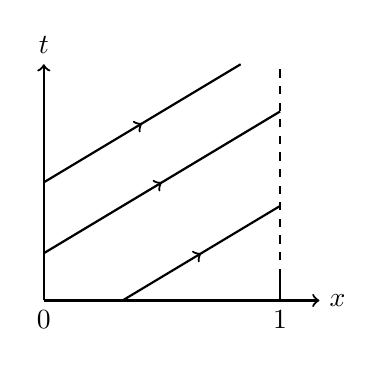
\begin{tikzpicture} 
   
\draw[->, thick] (0, 0) -- (3.5, 0) node[right] { $x$};
\draw[->, thick] (0, 0) -- (0, 3) node[above] { $t$};
 
 \draw  (0, 0)  node[below] { $0$};
  \draw  (3, 0)  node[below] { $1$};
  
  \draw[  thick,
        decoration={markings, mark=at position 0.5 with {\arrow{>}}},
        postaction={decorate}
        ]
        (0,1.5) -- (2.5, 3);
  
  
    \draw[  thick,
        decoration={markings, mark=at position 0.5 with {\arrow{>}}},
        postaction={decorate}
        ]
        (0,0.6) -- (3, 2.4);
  
   \draw[  thick,
        decoration={markings, mark=at position 0.5 with {\arrow{>}}},
        postaction={decorate}
        ]
        (1,0) -- (3, 1.2);
  
  
  \draw[thick, dashed] (3, 0.3) -- (3, 3);
  
\draw[thick] (3, 0) -- (3, 0.3);
  
    \end{tikzpicture}
 
\end{center}


$u(x, t)= \begin{cases}f(x-c t), & \text { if } x-c t>0 \\ g_{0}(t-x / c), & \text { if } x-c t<0\end{cases}$

\end{frame}





%-=-=-=-=-=-=-=-=-=-=-=-=-=-=-=-=-=-=-=-=-=-=-=-=
%	FRAME:
%-=-=-=-=-=-=-=-=-=-=-=-=-=-=-=-=-=-=-=-=-=-=-=-=
\begin{frame}{Advection equation: solution when $c<0$}


\begin{center}
	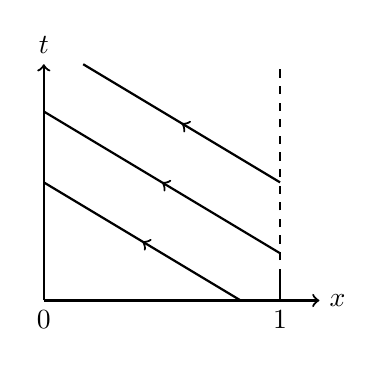
\begin{tikzpicture} 
   
\draw[->, thick] (0, 0) -- (3.5, 0) node[right] { $x$};
\draw[->, thick] (0, 0) -- (0, 3) node[above] { $t$};
 
 \draw  (0, 0)  node[below] { $0$};
  \draw  (3, 0)  node[below] { $1$};
  
  \draw[  thick,
        decoration={markings, mark=at position 0.5 with {\arrow{>}}},
        postaction={decorate}
        ]
(2.5, 0) -- (0, 1.5);
  
  
    \draw[  thick,
        decoration={markings, mark=at position 0.5 with {\arrow{>}}},
        postaction={decorate}
        ]
        (3, 0.6) -- (0, 2.4);
  
   \draw[  thick,
        decoration={markings, mark=at position 0.5 with {\arrow{>}}},
        postaction={decorate}
        ]
        (3,1.5) -- (0.5, 3);
  
  
  
  
  \draw[thick, dashed] (3, 0.3) -- (3, 3);
  
\draw[thick] (3, 0) -- (3, 0.3);
  
    \end{tikzpicture}
 
\end{center}


$u(x, t)= \begin{cases}f(x-c t), & \text { if } x-c t<1 \\ g_{1}(t-x /c ), & \text { if } x-c t>1\end{cases}$

\end{frame}







%-=-=-=-=-=-=-=-=-=-=-=-=-=-=-=-=-=-=-=-=-=-=-=-=
%	FRAME:
%-=-=-=-=-=-=-=-=-=-=-=-=-=-=-=-=-=-=-=-=-=-=-=-=
\begin{frame}{Advection equation: Method of line}


Consider $u_t + c u_x = 0$ with periodic BCs $u(0,t) = u(1,t)$.
\begin{center}
	    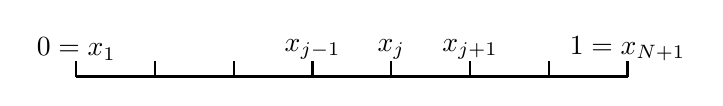
\begin{tikzpicture}
  \draw[color=black, thick] (0,0) -- (1, 0) -- (2, 0) -- (3, 0) -- (4, 0) -- (5, 0) -- (6, 0) -- (7, 0);
  \foreach \x in {0,...,7}
  {
  \draw[color=black, thick] (\x, 0) -- (\x, 0.2);
  }
  \node at (0, 0.35) {$0 = x_1$};
    \node at (7, 0.35) {$1 = x_{N+1}$};
     \node at (3, 0.35) {$ x_{j-1}$};
      \node at (4, 0.35) {$ x_{j}$};
       \node at (5, 0.35) {$x_{j+1}$};

\end{tikzpicture}
\end{center}


\vspace{0.5em}

BCs are $u_{N+1} = u_1$, and we need to solve for
$u_2, \ldots, u_{N+1}$. 
Then using our MoL equations from before:
\begin{align*}
\dot{u}_j(t) &= -\tfrac{c}{2h}(u_{j+1} - u_{j-1}), \\
\dot{u}_2(t) &= -\tfrac{c}{2h}(u_3 - u_1) = -\tfrac{c}{2h}(u_3 - u_{N+1}), \qquad \text{(not solving for $u_1$),} \\
\dot{u}_{N+1}(t) &= -\tfrac{c}{2h}(u_{N+2} - u_N) = -\tfrac{c}{2h}(u_2 - u_N), \qquad \text{(periodic BCs).} \\
\end{align*}

with initial condition $\dot{u}_j(0) = f(x_j)$.

\end{frame}





%-=-=-=-=-=-=-=-=-=-=-=-=-=-=-=-=-=-=-=-=-=-=-=-=
%	FRAME:
%-=-=-=-=-=-=-=-=-=-=-=-=-=-=-=-=-=-=-=-=-=-=-=-=
\begin{frame}{Advection equation: Method of line in matrix form}

Matrix form:
\begin{align*}
\dot{\mathbf{u}} &= A \mathbf{u},
\end{align*}
where the matrix $A$ is given by:
$$ A = -\frac{c}{2h} \left[ \begin{array}{ccccccc}
0 & 1 & \cdots & &  & 0& -1 \\
-1 & 0 & 1 & \cdots &  & 0 & 0 \\
0 & -1 & 0 & 1 & \cdots & 0 & 0  \\
\vdots \\
1 & 0 & 0 & 0 & \cdots & -1 & 0 
\end{array} \right]. $$

\end{frame}




%-=-=-=-=-=-=-=-=-=-=-=-=-=-=-=-=-=-=-=-=-=-=-=-=
%	FRAME:
%-=-=-=-=-=-=-=-=-=-=-=-=-=-=-=-=-=-=-=-=-=-=-=-=
\begin{frame}{Advection equation: eigenvalue of matrix}

 $A$ is skew-symmetric: $A^T = -A$! Its eigenvalues are imaginary.
$$ \lambda_p = -\frac{ic}{h} \sin(2\pi ph), \qquad p=1,\ldots,N. $$
Starts small, goes up and down. $\lambda_p \in [-ic/h, ic/h]$.


\vspace{0.5em}
For stability, we need to find time step, $k$, such that RAS for time stepper includes all $\lambda_p$.


\vspace{0.5em}

For FTCS, there is no $k$ which makes $|w^n|$ bounded as $n\rightarrow\infty$. FTCS is \emph{never
stable for the advection equation}. 



\end{frame}




%-=-=-=-=-=-=-=-=-=-=-=-=-=-=-=-=-=-=-=-=-=-=-=-=
%	FRAME:
%-=-=-=-=-=-=-=-=-=-=-=-=-=-=-=-=-=-=-=-=-=-=-=-=
\begin{frame}{Advection equation: leap frog method}

Leap frog method:
$$ \dot{u} = \frac{u^{n+1} - u^{n-1}}{2k}. $$
Its RAS is $|\mathfrak{Im}(z)| \le 1$. 
Leapfrog will be stable provided $$\lambda_k \in [-ick/h, ick/h] \subset [-i, i],$$
i.e. $\left| \frac{ck}{h} \right| < 1$.


\vspace{0.5em}


Courant Number: $\frac{ck}{h}=\nu$.  Condition on stability is $\nu < 1$.



\vspace{0.5em}

 Fully discrete leapfrog method (CTCS).
$$ u_j^{n+1} = u_j^{n-1} - \tfrac{ck}{h}(u_{j+1}^n - u_{j-1}^n). $$
This is an explicit method, $O(h^2, k^2)$. Three time levels means we need a
starting procedure and more memory.
 

\end{frame}



%-=-=-=-=-=-=-=-=-=-=-=-=-=-=-=-=-=-=-=-=-=-=-=-=
%	FRAME:
%-=-=-=-=-=-=-=-=-=-=-=-=-=-=-=-=-=-=-=-=-=-=-=-=
\begin{frame}{Advection equation: Lax-Friedrichs Method (LxF)}

For FTCS we had:
$$ u_j^{n+1} = u_j^n - \tfrac{\nu}{2}(u_{j+1}^n - u_{j-1}^n). $$


\vspace{0.5em}


If we replace $u_j^n$ with the average $\frac{1}{2}(u_{j+1}^n + u_{j-1}^n)$
we get LxF:
$$ u_j^{n+1} = \tfrac{1}{2}(u_{j+1}^n + u_{j-1}^n) - \tfrac{\nu}{2}(u_{j+1}^n - u_{j-1}^n). $$

\vspace{0.5em}

To do stability analysis, need to write as
$$ \dot{\mathbf{u}} = B\mathbf{u} $$


\end{frame}





%-=-=-=-=-=-=-=-=-=-=-=-=-=-=-=-=-=-=-=-=-=-=-=-=
%	FRAME:
%-=-=-=-=-=-=-=-=-=-=-=-=-=-=-=-=-=-=-=-=-=-=-=-=
\begin{frame}{Advection equation: Lax-Friedrichs Method (LxF)}


 $\frac{1}{2}(u_{j+1}^n + u_{j-1}^n)$ can be rewritten as \mbox{$u_j^n + \frac{1}{2}(u_{j+1}^n - 2u_j^n + u_{j-1}^n)$}, which is a diffusive (central difference of $u_{xx}$) term.
 
I.e., method adds artificial/numerical diffusion to stabilise the solution.


\vspace{0.5em}


Approximation of time derivative at $j$:
$$ u_j^{n+1} = u_j^n + \frac{1}{2}(u_{j+1}^n - 2u_j^n + u_{j-1}^n) - \tfrac{\nu}{2}(u_{j+1}^n - u_{j-1}^n) $$

In matrix form
$$ \frac{\mathbf{u}^{n+1} - \mathbf{u}^n}{k} = \tfrac{1}{2k}A_{+}\mathbf{u} -\tfrac{c}{2h}A_{-}\mathbf{u} = B\mathbf{u}. $$


where $A_+$ is symmetric and $A_-$ is skew-symmetric.


\end{frame}








%-=-=-=-=-=-=-=-=-=-=-=-=-=-=-=-=-=-=-=-=-=-=-=-=
%	FRAME:
%-=-=-=-=-=-=-=-=-=-=-=-=-=-=-=-=-=-=-=-=-=-=-=-=
\begin{frame}{Advection equation: Lax-Friedrichs Method (LxF)}
Eigenvalues of $B$: $-\frac{ic}{h}\sin(2\pi ph)-\frac{1}{k}(1-cos(2\pi ph)) = \lambda_p$.


\vspace{0.5em}


At time step $k$, $k\lambda_p = -i\nu\sin(2\pi ph) - (1 - cos(2\pi ph)$ which lie on
an ellipse.


\vspace{0.5em}


Since $p$ is a real number,
$$ k\lambda_p = -\underbrace{i \nu \sin(2\pi p h)}_\text{imaginary} - \underbrace{(1 - cos(2\pi p h))}_\text{real}. $$

So $k\lambda_p$ in RAS if $|k\lambda_p + 1| < 1$, i.e. $ \nu^2\sin^2(2\pi ph) + \cos^2(2\pi ph)< 1$ $\Rightarrow |\nu|< 1$. 



\vspace{0.5em}



LxF is stable iff $|\nu| < 1$. But it is only 1st order in time, $\text{LTE} = \mathcal{O}(k,h^2)$.




\end{frame}





%-=-=-=-=-=-=-=-=-=-=-=-=-=-=-=-=-=-=-=-=-=-=-=-=
%	FRAME:
%-=-=-=-=-=-=-=-=-=-=-=-=-=-=-=-=-=-=-=-=-=-=-=-=
\begin{frame}{Advection equation: Lax-Wendroff Method (LxW)}
To get a 2nd order method, use  Taylor series expansion on PDE
\begin{align*}
u(x,t+k) &= u(x,t) + k u_t(x,t) + \tfrac{1}{2} k^2 u_{tt}(x, t) + O(k^3), \\
u_t &= -c u_x, \qquad u_{tt} = c^2 u_{xx}, \\
\Longrightarrow \quad u(x,t+k) &= u(x,t) - k c \underbrace{u_x}_\text{CD} +\frac{k^2 c^2}{2} \underbrace{u_{xx}}_{\text{CD}} +\ O(k^3), \\
\Longrightarrow \quad u_j^{n+1} &= u_j^n - \tfrac{\nu}{2}(u_{j+1}^n - u_{j-1}^n) 
        + \tfrac{\nu^2}{2}(u_{j+1}^n - 2u_j^n + u_{j-1}^n),
\end{align*}

\vspace{0.5em}


$\dot{\mathbf{u}} = B\mathbf{u}$ evolves the system and:
$$k\lambda_p = -i\left(\tfrac{ck}{h}\right)\sin(\pi p h) + \left(\tfrac{ck}{h}\right)^2(\cos(\pi p h) - 1),
\qquad p=1,\ldots,N. $$
It is stable if  $|\nu| \le 1$ and $\text{LTE} = \mathcal{O}(k^2,h^2)$.

\end{frame}







%-=-=-=-=-=-=-=-=-=-=-=-=-=-=-=-=-=-=-=-=-=-=-=-=
%	FRAME:
%-=-=-=-=-=-=-=-=-=-=-=-=-=-=-=-=-=-=-=-=-=-=-=-=
\begin{frame}{Advection equation: upwind method}
The advection equation has a direction:
\begin{itemize}
	\item If~$c>0$, information comes from the left. 
	\item If~$c < 0$, information comes from the right.
\end{itemize}

\vspace{0.5em}

Use 1-sided FD, depending on sign of~$c$. This gives us ``upwind methods'':
use FTBS for~$c > 0$ and use FTFS for~$c < 0$.


\begin{equation*}
u_j^{n+1} = \left\{ \begin{array}{ll} 
    u_j^n - \nu(u_j^n - u_{j-1}^{n}), & \text{if}\ c > 0 \\
    u_j^n - \nu(u_{j+1}^n - u_j^n), & \text{if}\ c < 0
\end{array} \right.
\end{equation*}


\end{frame}


%-=-=-=-=-=-=-=-=-=-=-=-=-=-=-=-=-=-=-=-=-=-=-=-=
%	FRAME:
%-=-=-=-=-=-=-=-=-=-=-=-=-=-=-=-=-=-=-=-=-=-=-=-=
\begin{frame}{Advection equation: stability of upwind method}

FTBS stable for $0 < \nu < 1$ ($c>0$ only). 

\vspace{0.5em}

FTFS stable for $-1 < \nu < 0$ ($c < 0$ only).

\vspace{0.5em}

FTBS and FTFS have $\text{LTE} = O(k, h)$.

\vspace{0.5em}

Even though lower accuracy than Lax-Wendroff Method it can often perform better if discontinuities are present in solution.

\end{frame}





%-=-=-=-=-=-=-=-=-=-=-=-=-=-=-=-=-=-=-=-=-=-=-=-=
%	FRAME:
%-=-=-=-=-=-=-=-=-=-=-=-=-=-=-=-=-=-=-=-=-=-=-=-=
\begin{frame}{Advection equation: Beam-Warming method}
To get 2nd order method, use 1-sided 2nd order FD in Lax-Wendroff method, 


\begin{align*}
u_j^{n+1} &= \left\{ \begin{array}{ll} 
    u_j^n - \frac{\nu}{2}(3u_j^n - 4u_{j-1}^{n} + u^n_{j-2}) + 
    \frac{\nu^2}{2}(u_j^n - 2u_{j-1}^{n} + u^n_{j-2}), & \text{if}\ c > 0 \\
    u_j^n -  \frac{\nu}{2}(-3u_j^n + 4u_{j+1}^{n} - u^n_{j+2}) + 
    \frac{\nu^2}{2}(u_j^n - 2u_{j+1}^{n} + u^n_{j+2}), & \text{if}\ c < 0
\end{array} \right.
\end{align*}

Stable when $0\le\nu \le 2$ if $c>0$ and $-2\le \nu \le 0$ if $c\le 0$.

\end{frame}










%-=-=-=-=-=-=-=-=-=-=-=-=-=-=-=-=-=-=-=-=-=-=-=-=
%	FRAME:
%-=-=-=-=-=-=-=-=-=-=-=-=-=-=-=-=-=-=-=-=-=-=-=-=
\begin{frame}{Advection equation: analytical domain of dependence}


Domain of dependence of analytical solution: $D \subseteq \mathbb{R}$ is the smallest region such that $u(x,t)$ depends only on the values of $f(x)$ where $x\in D$.

 
 \begin{center}

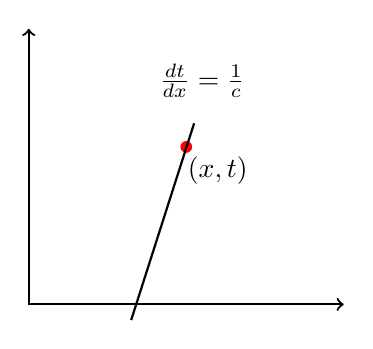
\begin{tikzpicture}

\draw [<->, black, thick] (0,3.5) --(0,0)-- (4, 0);


               \node at (2, 2)[circle,fill=red,inner sep=1.5pt]{};

\draw [black, thick] (1.3, -0.2) -- (2.1, 2.3);

 \node  at (2.2, 2.5) [above]   {$\frac{dt}{dx}=\frac{1}{c}$};

 \node  at (2.4, 2) [below]   {$(x, t)$};


    \end{tikzpicture}
    
    \vspace{0.5em}
\centering{ Analytic}
 

	
\end{center}

We therefore have $D = \{x - ct\}$; i.e., solution at $u(x, t)$ only depends on $f(x-ct)$ (because all information travels along a characteristic with no diffusion).
 
 
 
 
  
  
\end{frame}





%-=-=-=-=-=-=-=-=-=-=-=-=-=-=-=-=-=-=-=-=-=-=-=-=
%	FRAME:
%-=-=-=-=-=-=-=-=-=-=-=-=-=-=-=-=-=-=-=-=-=-=-=-=
\begin{frame}{Advection equation: numerical domain of dependence}
 

Domain of dependence of numerical solution: $D_h \subseteq \mathbb{R}$ is the smallest region such that $u^n_j$ depends only on the values of $f(x_j)$ where $x_j \in D_h$.

 \begin{columns}
 
\begin{column}{.5\textwidth}
	

\begin{center}
Upwind scheme

\vspace{0.5em}
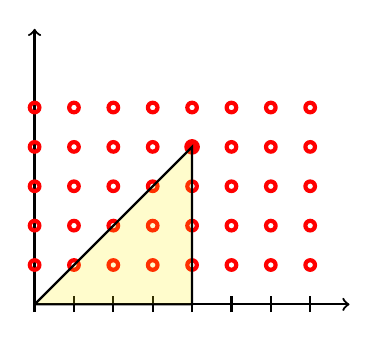
\begin{tikzpicture}
	\draw [<->, black, thick] (0,3.5) --(0,0)-- (4, 0);

\foreach \x in {0,...,7}
    \foreach \y [count=\yi] in {1,...,5}  
      \draw[draw=none,fill=red, even odd rule]   (0.5*\x, 0.5*\y) circle(2.5pt) circle(1.0pt);

\foreach \x in {0,...,7}
     \draw [black, thick](0.5*\x, -0.1) -- (0.5*\x, 0.1);


               \node at (2, 2)[circle,fill=red,inner sep=2.0pt]{};

\draw [fill=yellow, fill opacity = 0.2, thick] (0, 0) -- (2, 0) -- (2,2) -- (0, 0);

\end{tikzpicture}
\vspace{0.5em}
\centering{Numerical }

	
\end{center}

\end{column}

\begin{column}{.5\textwidth}

\begin{center}
LxW scheme

\vspace{0.5em}
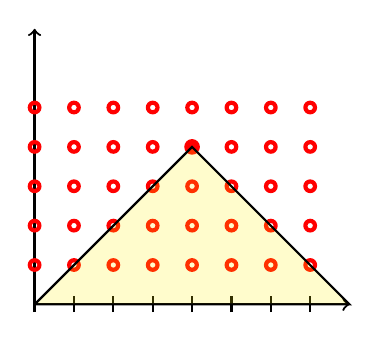
\begin{tikzpicture}
	\draw [<->, black, thick] (0,3.5) --(0,0)-- (4, 0);

\foreach \x in {0,...,7}
    \foreach \y [count=\yi] in {1,...,5}  
      \draw[draw=none,fill=red, even odd rule]   (0.5*\x, 0.5*\y) circle(2.5pt) circle(1.0pt);

\foreach \x in {0,...,7}
     \draw [black, thick](0.5*\x, -0.1) -- (0.5*\x, 0.1);


               \node at (2, 2)[circle,fill=red,inner sep=2.0pt]{};

\draw [fill=yellow, fill opacity = 0.2, thick] (0, 0) -- (4, 0) -- (2,2) -- (0, 0);

\end{tikzpicture}
\vspace{0.5em}
\centering{Numerical }

	
\end{center}
\end{column}


\end{columns}



\end{frame}








%-=-=-=-=-=-=-=-=-=-=-=-=-=-=-=-=-=-=-=-=-=-=-=-=
%	FRAME:
%-=-=-=-=-=-=-=-=-=-=-=-=-=-=-=-=-=-=-=-=-=-=-=-=
\begin{frame}{Advection equation: numerical domain of dependence}

Define $r = k/h$. From the numerical schemes we can calculate
 

$$D_h = \left(X + p\frac{T}{r}, X + q\frac{T}{r}\right).$$ 

\vspace{0.5em}



 LxW has $p=-1, q=1$ so domain of dependence is 
$$D_h = \left(X-\frac{T}{r}, X+\frac{T}{r}\right).$$ 

\vspace{0.5em}


UW $(c>0)$ has $p=-1, q=0$ so domain of dependence is 
$$D_h = \left(X - \frac{T}{r}, X\right).$$

 
  
\end{frame}


%-=-=-=-=-=-=-=-=-=-=-=-=-=-=-=-=-=-=-=-=-=-=-=-=
%	FRAME:
%-=-=-=-=-=-=-=-=-=-=-=-=-=-=-=-=-=-=-=-=-=-=-=-=
\begin{frame}{Advection equation: CFL condition}

\alert{CFL (Courant-Friedrichs-Lewy) condition}: Necessary condition for convergence as $h,k \rightarrow 0$ of a numerical method for an advection equation is that
$$ D \subseteq D_h $$

If $D \nsubseteq D_h$ then information from the initial condition would not propagate forwards to the correct location.

\vspace{0.5em}


For UW and LxW we have
\begin{equation*}
	\begin{split}
		&X-cT \in [X + pT/r, X + qT/r]\\
		\Rightarrow \quad & pT/r \le -cT \le qT/r\\
		\Rightarrow \quad & -q\le cr = \nu \le -p
	\end{split}
\end{equation*}
  
I.e., CFL gives same condition as stability.
  
\end{frame}


\begin{frame}{Visualisation of CFL condition}



 
 \begin{columns}
 
\begin{column}{.5\textwidth}
\begin{center}

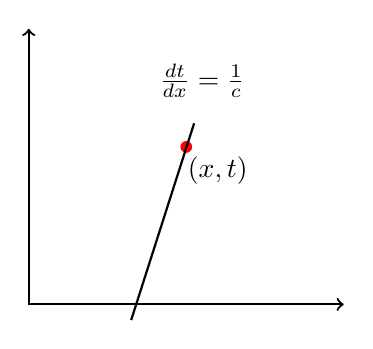
\begin{tikzpicture}

\draw [<->, black, thick] (0,3.5) --(0,0)-- (4, 0);


               \node at (2, 2)[circle,fill=red,inner sep=1.5pt]{};

\draw [black, thick] (1.3, -0.2) -- (2.1, 2.3);

 \node  at (2.2, 2.5) [above]   {$\frac{dt}{dx}=\frac{1}{c}$};

 \node  at (2.4, 2) [below]   {$(x, t)$};


    \end{tikzpicture}
    
    \vspace{0.5em}
\centering{ Analytic}
 

	
\end{center}

\end{column}%
 
 \begin{column}{.5\textwidth}

\begin{center}
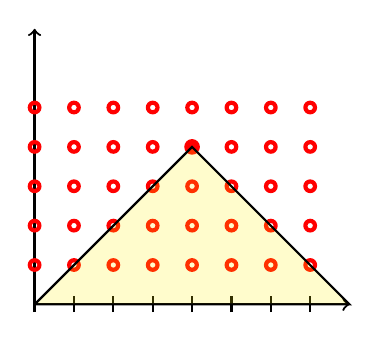
\begin{tikzpicture}
	\draw [<->, black, thick] (0,3.5) --(0,0)-- (4, 0);

\foreach \x in {0,...,7}
    \foreach \y [count=\yi] in {1,...,5}  
      \draw[draw=none,fill=red, even odd rule]   (0.5*\x, 0.5*\y) circle(2.5pt) circle(1.0pt);

\foreach \x in {0,...,7}
     \draw [black, thick](0.5*\x, -0.1) -- (0.5*\x, 0.1);


               \node at (2, 2)[circle,fill=red,inner sep=2.0pt]{};

\draw [fill=yellow, fill opacity = 0.2, thick] (0, 0) -- (4, 0) -- (2,2) -- (0, 0);

\end{tikzpicture}
\vspace{0.5em}
\centering{Numerical }

	
\end{center}
\end{column}


\end{columns}


	
\end{frame}






%-=-=-=-=-=-=-=-=-=-=-=-=-=-=-=-=-=-=-=-=-=-=-=-=
%	FRAME:
%-=-=-=-=-=-=-=-=-=-=-=-=-=-=-=-=-=-=-=-=-=-=-=-=
\begin{frame}{Advection equation: CFL condition for LxW scheme}


\begin{center}

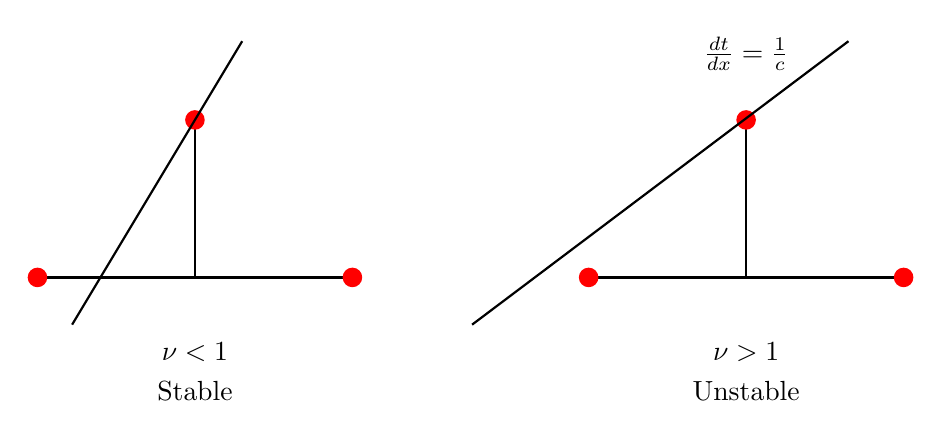
\begin{tikzpicture}

\draw[black, thick] (0, 0) -- (4, 0);
\draw[black, thick] (2, 0) -- (2, 2);

   \node at (0, 0)[circle,fill=red,inner sep=2.5pt]{};

   \node at (2, 2)[circle,fill=red,inner sep=2.5pt]{};
   \node at (4, 0)[circle,fill=red,inner sep=2.5pt]{};

\draw [black, thick] (0.44, -0.6) -- (2.6, 3);

 \node  at (2, -0.7) [below]   {$\nu < 1$};
 
  \node  at (2, -1.2) [below]   {Stable};

 
 
 \draw[black, thick] (7, 0) -- (11, 0);
\draw[black, thick] (9, 0) -- (9, 2);

   \node at (7, 0)[circle,fill=red,inner sep=2.5pt]{};

   \node at (9, 2)[circle,fill=red,inner sep=2.5pt]{};
   \node at (11, 0)[circle,fill=red,inner sep=2.5pt]{};

\draw [black, thick] (5.52, -0.6) -- (10.3, 3);

 \node  at (9, -0.7) [below]   {$\nu > 1$};
 
  \node  at (9, 2.5) [above]   {$\frac{dt}{dx}=\frac{1}{c}$};


  \node  at (9, -1.2) [below]   {Unstable};

    \end{tikzpicture}
    
    
    
    
    
    
    
    \vspace{0.5em}

 

	
\end{center}




  
\end{frame}



%-=-=-=-=-=-=-=-=-=-=-=-=-=-=-=-=-=-=-=-=-=-=-=-=
%	FRAME:
%-=-=-=-=-=-=-=-=-=-=-=-=-=-=-=-=-=-=-=-=-=-=-=-=
\begin{frame}{Advection equation: examples of CFL condition}

\begin{center}
\resizebox{0.9\textwidth}{!}{
 \begin{tabular}{llll}
    LxF & 
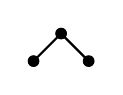
\begin{tikzpicture}
         \node at (0, 0)[circle,fill,inner sep=1.5pt]{};
           \node at (0.70, 0)[circle,fill,inner sep=1.5pt]{};
         \node at (0.35,0.35)[circle,fill,inner sep=1.5pt]{};
         \draw [black, thick] (0,0) -- (0.35, 0.35) --(0.70,0) ;
    \end{tikzpicture}
  & $p=-1,q=1$ & $-1\le \nu \le 1$\\
  LxW&
  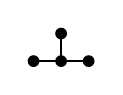
\begin{tikzpicture}
  \node at (0, 0)[circle,fill,inner sep=1.5pt]{};
           \node at (0.70, 0)[circle,fill,inner sep=1.5pt]{};
                    \node at (0.35,0)[circle,fill,inner sep=1.5pt]{};
         \node at (0.35,0.35)[circle,fill,inner sep=1.5pt]{};
         \draw [black, thick] (0,0)  --(0.70,0) ;
         \draw [black, thick] (0.35, 0.35) -- (0.35, 0);
    \end{tikzpicture}
  & $p=-1,q=1$ & $-1\le \nu \le 1$\\
   UW&
  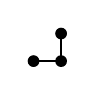
\begin{tikzpicture}
  \node at (0, 0)[circle,fill,inner sep=1.5pt]{};
           \node at (0.35, 0)[circle,fill,inner sep=1.5pt]{};
         \node at (0.35,0.35)[circle,fill,inner sep=1.5pt]{};
         \draw [black, thick] (0,0)  --(0.35,0) ;
         \draw [black, thick] (0.35, 0.35) -- (0.35, 0);
    \end{tikzpicture}
  & $p=-1,q=0$ & $0\le \nu \le 1$\\
   UW&
  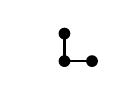
\begin{tikzpicture}
   \node at (0, 0){};
  \node at (0.35, 0)[circle,fill,inner sep=1.5pt]{};
           \node at (0.70, 0)[circle,fill,inner sep=1.5pt]{};
         \node at (0.35,0.35)[circle,fill,inner sep=1.5pt]{};
         \draw [black, thick] (0.35,0)  --(0.70,0) ;
         \draw [black, thick] (0.35, 0.35) -- (0.35, 0);
    \end{tikzpicture}
  & $p=0, q=1$ & $-1\le \nu \le 0$\\
     BW&
  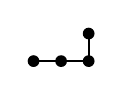
\begin{tikzpicture}
  \node at (0, 0)[circle,fill,inner sep=1.5pt]{};
         \node at (-0.7, 0)[circle,fill,inner sep=1.5pt]{};
         \node at (0,0.35)[circle,fill,inner sep=1.5pt]{};
         \node at (-0.35,0)[circle,fill,inner sep=1.5pt]{};
         \draw [black, thick] (0,0)  --(-0.35,0) ;
         \draw [black, thick] (0, 0) -- (0, 0.35);
         \draw [black, thick] (-0.35, 0) -- (-0.7, 0);
    \end{tikzpicture}
  & $p=-2,q=0$ & $0\le \nu \le 2$\\
       BW&
  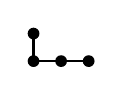
\begin{tikzpicture}
  \node at (0, 0)[circle,fill,inner sep=1.5pt]{};
         \node at (0.35, 0)[circle,fill,inner sep=1.5pt]{};
         \node at (-0.35,0.35)[circle,fill,inner sep=1.5pt]{};
         \node at (-0.35,0)[circle,fill,inner sep=1.5pt]{};
         \draw [black, thick] (0,0)  --(0.35,0) ;
         \draw [black, thick] (-0.35, 0.35) -- (-0.35, 0);
         \draw [black, thick] (0.35, 0) -- (-0.35, 0);
    \end{tikzpicture}
  & $p=0,q=2$ & $-2\le \nu \le 0$\\
    \end{tabular}}
\end{center}
  But not sufficient
  
  
  \begin{center}
\resizebox{0.97\textwidth}{!}{
 \begin{tabular}{llll}
    FTCS & 
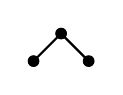
\begin{tikzpicture}
         \node at (0, 0)[circle,fill,inner sep=1.5pt]{};
           \node at (0.70, 0)[circle,fill,inner sep=1.5pt]{};
         \node at (0.35,0.35)[circle,fill,inner sep=1.5pt]{};
         \draw [black, thick] (0,0) -- (0.35, 0.35) --(0.70,0) ;
    \end{tikzpicture}
  & $\Rightarrow |\nu|\le 1$ from CFL condition  & but not stable for any $\nu$ \\

    \end{tabular}}
\end{center}
\end{frame}







%-=-=-=-=-=-=-=-=-=-=-=-=-=-=-=-=-=-=-=-=-=-=-=-=
%	FRAME:
%-=-=-=-=-=-=-=-=-=-=-=-=-=-=-=-=-=-=-=-=-=-=-=-=
\begin{frame}[standout]
  End of week 9!
\end{frame}

\appendix



\end{document}
